\documentclass[a4paper,11pt]{scrartcl}

\usepackage[utf8]{inputenc}
\usepackage[ngerman]{babel}
\usepackage[T1]{fontenc}
\usepackage{amsmath}
\usepackage{graphicx}
\usepackage{tabularx}
\usepackage[a4paper, left=2cm, right=2cm, top=2.8cm, bottom=2.8cm]{geometry}
\usepackage{tikz}   
\usepackage[scaled]{helvet}
\usepackage{tabto} 
\usepackage{fancyhdr}
\usepackage{multirow}

\renewcommand*{\familydefault}{\sfdefault}

\pagestyle{fancy}

\setkomafont{section}{\huge}
\setkomafont{subsection}{\Large}


\lhead{Maximilian Hoffmann}
\chead{Betrieblicher Auftrag \\ \textbf{Kabeltester}}
\rhead{
\includegraphics[width=3cm]{Bilder/BMK_LOGO.png}}

\begin{document}

\section{Blockschaltbild}
	
\begin{center}
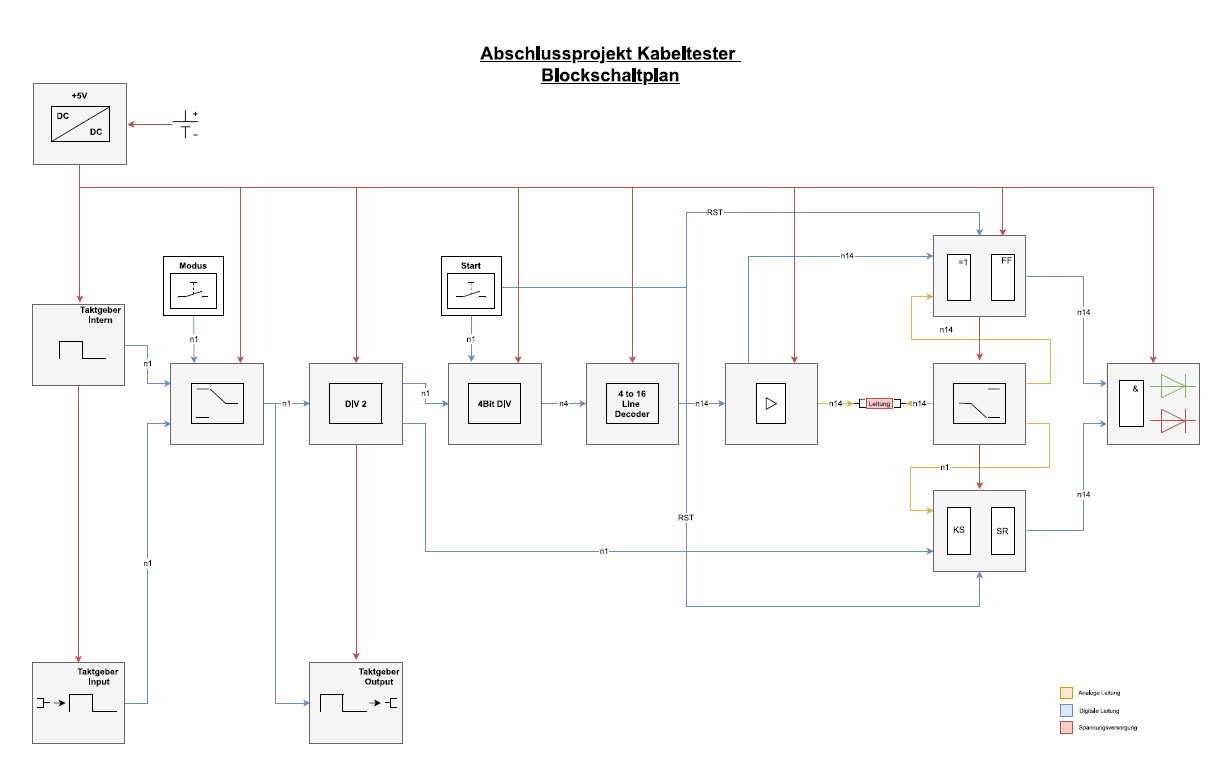
\includegraphics[width=22cm, angle=-90]{Bilder/Blockschaltplan.png}
\end{center}

\newpage

\begin{center}
Die Kernfunktion der Messplatine wird in diesem Dokumentationsteil anhand des Blockschaltbildes erklärt. 
\end{center}

Die Versorgung dieser Platine soll durch einen 9V Batterieblock erfolgen. Die Spannung wird dabei durch einen DC/DC - Wandler auf 5V gewandelt.
\\
\\
Ein interner sowie externen Takt kann Wahlweise als Systemtakt verwendet werden. Mit einem Taster wird zwischen diesen Taktquellen umgeschaltet.
\\
\\
Um den Systemtakt auf mehreren hintereinander geschalteten Messplatinen verwenden zu können, wird dieser über einen Stecker herausgeführt.
\\
\\
Der Systemtakt wird nun durch den Faktor zwei geteilt und bildet den Messtakt. Synchron zu diesen Takt werden die einzelnen Adern geprüft.
\\
\\
Um jede einzelne Ader nach einander messen zu können, wird mit Hilfe des Messtaktes, durch einen 4 Bit Zählerbaustein von 0 bis 15 hochgezählt. Über einen Taster wird der Zählvorgang gestartet.
\\
\\
Der 4Bit Decoder schaltet dabei für jeden möglichen Zählerstand den passenden Ausgang auf High. Läuft keine Messung, so weißen alle Ausgänge ein Low-Pegel auf. 
\\
\\
Da bei der Konstantstrommessung ein Strom bis zu 100mA durch das Kabel fließen kann, steuert der 4 Bit Decoder mit seinen Ausgängen die Leistungsstufen an.
\\
\\
Zwischen den Leistungsstufen und dem Analogschalter wird das zu Messende Kabel  (Ader) gesteckt. 
\\
\\
Der Analogschalter ist dafür verantwortlich zwischen der Konstantstrommessung und der Kurzschlussmessung sowie Durchgangsmessung, während der Prüfung umzuschalten. 
\\
\\
Während der Pausenzeit des Messtaktes, wird ein konstanter Strom durch das Kabel fließen. Mit Hilfe des Spannungsfall über den strombegrenzenden MOSFET der Konstantstromquelle, kann indirekt der Kabelwiderstand bestimmt werden. Das Ergebnis dieser seriellen Messung wird durch ein Schieberegister parallel ausgegeben. Da die Konstantstromquelle bei jedem Kabel den Strom neu regeln muss, wird durch den zugeführten Systemtakt erst nach der Hälfte der Messzeit das Ergebnis via Schiebetakt übernommen.
\\
\\
Während der Impulszeit des Messtaktes, wird das Kabel auf Kurschluss sowie Durchgängigkeit überprüft. 
\\
\\
Liefern beide Messungen einer Ader ein High-Signal, leuchtet eine grüne LED. Liefert eine oder beide Messungen ein Low-Signal, leuchtet die rote LED.




\end{document}